\documentclass[11pt]{article}
\usepackage[margin=1in]{geometry}
\usepackage[T1]{fontenc}
\usepackage{amsmath,amssymb}
\usepackage{graphicx}
\usepackage{booktabs,tabularx,longtable,array}
\usepackage{xcolor}
\usepackage{tikz}
\usetikzlibrary{arrows.meta,positioning,calc}
\usepackage[numbers,sort&compress]{natbib}
\usepackage[hidelinks]{hyperref}
\usepackage{xurl}
\usepackage{enumitem}
\usepackage{caption}
\usepackage[most]{tcolorbox}
\setlist{itemsep=2pt,topsep=4pt}
\captionsetup{font=small,labelfont=bf}
\definecolor{nb}{HTML}{2A78D6}\definecolor{sb}{HTML}{EB6834}\definecolor{gr}{HTML}{1BAF7A}
\definecolor{ink}{HTML}{1D2622}\definecolor{muted}{HTML}{6B736E}\definecolor{acc}{HTML}{0F6E66}
\newcolumntype{L}{>{\raggedright\arraybackslash}X}
\graphicspath{{figures/}}
\newtcolorbox{keybox}[1]{colback=acc!5,colframe=acc!60,fonttitle=\bfseries,title=#1,boxrule=0.6pt,arc=2pt}
\newcommand{\flag}[1]{\textcolor{sb}{\textsf{[#1]}}}

\title{The River LINE in Context:\\
\large Riders, Community Effects, History, Money, What Went Wrong, What Worked, and What Is Planned}
\author{ISE Senior Design Team 22 \quad (faculty advisor: R.~Hildebrand)\\Grado Department of Industrial and Systems Engineering, Virginia Tech}
\date{Background report --- September 28, 2026}

\begin{document}
\maketitle

\begin{abstract}
This report collects what is publicly known about NJ TRANSIT's River LINE beyond its timetable: who rides it and how satisfied they are, what it has done for the towns along it, how it was built and changed, what it costs, what went wrong and what worked, how similar systems have fared, and what is planned. Each statement is cited, and sources are graded as official, academic, news, advocacy, or Wikipedia. The main findings are these.
\begin{itemize}
\item Riders rated the River LINE lowest of NJ TRANSIT's three light rail lines in every survey wave from 2022 to 2025. Its score fell from 6.6 out of 10 (Spring 2022) to 5.9 (Spring 2025), then jumped to 6.8 in Fall 2025 after the takeover was announced.
\item The line cost about \$1.1 billion in state money. It carried 2.65 million trips in 2019 and 1.63 million in 2025, and covers only about 3\% of its operating cost from fares.
\item Its measured effect on property values and development has been modest.
\item Reliability collapsed in 2022--2025: the fleet went from 22{,}337 to 4{,}192 miles between failures. NJ TRANSIT took over operations from Alstom on February 14, 2026. Since then on-time performance has stayed above 93\%, and ridership in June--July 2026 was 12--22\% above a year earlier.
\item No extension is funded. The fleet is to be rebuilt or replaced within five to seven years, and the proposed Glassboro--Camden Line would meet the River LINE in Camden.
\end{itemize}
The report ends with what these facts mean for our schedule-optimization project and a companion list of documents we could not fully download.
\end{abstract}

\tableofcontents
\newpage

%======================================================================
\section{Summary}
\begin{keybox}{Ten things to know}
\begin{enumerate}[leftmargin=*]
\item \textbf{Riders were unhappy, and are less so since the takeover.} The line scored lowest among NJ TRANSIT's light rail lines in every wave from 2022 to 2025, bottoming at 5.9/10 in Spring 2025. It rose to 6.8 in Fall 2025, close to Hudson--Bergen and Newark Light Rail (both 7.0) \citep{njtcss2025fall}. In the 2010 DVRPC survey, customer communication was the lowest-rated attribute \citep{dvrpc2013}.
\item \textbf{Riders depend on it.} In 2010, 63\% rode to work, 21\% had no vehicle, and 21\% had household incomes under \$25{,}000 \citep{dvrpc2013}.
\item \textbf{Ridership has not recovered.} There were 2.65 million trips in 2019 and 1.63 million in 2025, or 61\% of 2019 \citep{ntd_monthly}. The other NJ TRANSIT light rail lines are at 94--99\% \citep{njtod2026}.
\item \textbf{It costs about \$20 per trip to run} and earns about \$0.46 per trip in fares: \$36.4 million in operating cost and 2.6\% farebox recovery in FY2024 \citep{ntd_metrics2224,ols2026njt}.
\item \textbf{The development effects have been modest.} The Rutgers evaluations found ``modest and mixed'' economic effects and neutral to slightly negative effects on home values \citep{chatman2010,chatman2012}. Only 35\% of land near stations is in transit-supportive use \citep{njtod2026}.
\item \textbf{The fleet is the core problem.} The 20 Stadler cars date from 2002--03. Miles between failures fell from 22{,}337 (2022) to 4{,}192 (2024) \citep{roinj2025}. Parts, auxiliary power units, and engines have been the bottlenecks \citep{inquirer2023,njt2024interim,centraljersey2025}.
\item \textbf{The operator changed in 2026.} NJ TRANSIT ended Alstom's contract effective February 13, 2026 and has run the line since February 14, with Kinkisharyo maintaining the vehicles. In-house operation costs \$40.6 million a year, \$3.1 million more than the contract \citep{ols2027njt}.
\item \textbf{Early results are good.} On-time performance has stayed above 93\% since the takeover, against about 87\% in 2024--25 \citep{ols2027njt}. June and July 2026 ridership was 22\% and 12\% above the same months of 2025 \citep{ntd_monthly}.
\item \textbf{Safety.} An operator was killed when a train struck a fallen tree near Florence on October 14, 2024 \citep{ntsb2025}, and there have been pedestrian deaths at crossings \citep{singleton2025}.
\item \textbf{The future is fleet renewal, not extension.} NJ TRANSIT says it will rebuild or replace the whole fleet within 5--7 years \citep{centraljersey2025}, and a replacement RFP was ``in development'' in January 2026 \citep{njt2026rehab}. No extension is funded. The Glassboro--Camden Line (about \$2 billion, only \$200 million secured) would connect at Walter Rand \citep{inquirer2026gcl}.
\end{enumerate}
\end{keybox}

%======================================================================
\section{Scope and sources}
The report answers five questions:
\begin{enumerate}
\item How do riders rate the River LINE?
\item What has it done, and what could better transit do, for the towns it serves and for riders' well-being?
\item When was it built and last updated?
\item What does it cost, and who pays?
\item What went wrong, what worked, and what is planned?
\end{enumerate}
We searched official sources first: NJ TRANSIT press releases, New Jersey Office of Legislative Services (OLS) budget analyses, the National Transit Database (NTD), the NTSB, the FRA, and DVRPC and NJTPA planning documents. We then used academic studies, major newspapers and trade press, and advocacy organizations. Wikipedia is used only where marked \flag{W}.

Several key documents could not be read in full because they sit behind robots rules, JavaScript dashboards, or paywalls. They are listed with URLs in the companion \emph{Documents to Download}. Figures that we read only through an automated summarizer are marked \flag{verify}.

\begin{table}[ht]\centering\small
\begin{tabularx}{\textwidth}{@{}lL@{}}
\toprule
Grade & Examples used here \\
\midrule
Official (P) & NJ TRANSIT releases; OLS budget analyses; NTD data; NTSB; FRA; DVRPC and NJTPA TIPs; NJDOT \\
Academic (A) & Rutgers Voorhees Transportation Center; peer-reviewed journals \\
News (N) & Philadelphia Inquirer, NJ.com, News 12, CBS Philadelphia, ROI-NJ, Railway Gazette, Mass Transit \\
Advocacy (V) & NJTOD newsletter, Tri-State Transportation Campaign, Reason Foundation \\
Wikipedia (W) & Only where no primary source was found; flagged \\
\bottomrule
\end{tabularx}
\caption{How sources are graded in this report.}
\end{table}

%======================================================================
\section{The line at a glance}
\begin{table}[ht]\centering\small
\begin{tabularx}{\textwidth}{@{}p{4.2cm}L@{}}
\toprule
Route & Entertainment Center (Camden) to Trenton Transit Center, about 34 miles, 21 stations, along the Delaware River \citep{njt_rline}. \\
Track & Former Conrail Bordentown Secondary, bought by NJ TRANSIT in 1999 for \$67.5 million \flag{W}. Mostly single track with passing sidings. Freight runs at night under FRA ``temporal separation'' \citep{fr1999waiver,fra2005horn}. \\
Vehicles & 20 Stadler GTW 2/6 diesel light rail cars (\#3501--3520), delivered 2002--03 with Bombardier (formerly Adtranz) \citep{pesky2025,nj_sso2021}. \\
Shops and storage & Main shop and control center: Camden Light Rail Complex. Burlington City Yard holds 2 cars overnight; the Trenton Layover Facility holds 8 \citep{nj_sso2021}. \\
Infrastructure & 72 grade crossings, 23 rail bridges, automatic block signals; shared with Conrail freight from MP 4.5 (Pennsauken) to MP 32.9 (Trenton); trains limited to 2 cars by platform length \citep{nj_sso2021}. \\
Opened & March 14, 2004 \citep{camdenhistory2004,njt_rline}. \\
Service & 15-minute peaks (from 2004) and 30-minute off-peak; roughly 6\,am--10\,pm \citep{njt2004fifteen,njt2003debut}. \\
Fare & \$1.90 base; \$0.85 reduced \citep{njt_fares}. \\
Operator & 2004--2015: Southern New Jersey Rail Group (Bechtel/Adtranz, then Bombardier). 2015--2026: Bombardier, Alstom from 2021. Since February 14, 2026: NJ TRANSIT, with Kinkisharyo for vehicle maintenance \citep{ols2027njt}. \\
NTD reporting & NTD reports the line as \emph{Hybrid Rail} (mode YR), not light rail: purchased transportation through February 2026, directly operated after \citep{ntd_monthly}. \\
\bottomrule
\end{tabularx}
\caption{The River LINE in brief.}
\end{table}

The NTD classification corrects our earlier data work. The main report and data-sources document said the River LINE was reported together with Hudson--Bergen. In fact the ``light rail, purchased transportation'' row is Hudson--Bergen alone, and the River LINE has its own Hybrid Rail row. This gives us River LINE-specific cost, ridership, and service data (Sections~\ref{sec:ridership} and \ref{sec:money}).

%======================================================================
\section{History and timeline}\label{sec:history}
\subsection{Origins and construction}
NJ TRANSIT began planning a South Jersey light rail line in the early 1990s. In 1996 its board chose a diesel light rail line on the Bordentown Secondary freight corridor \flag{W}. In December 1998 a Bechtel--Adtranz team was named low bidder for a design--build--operate--maintain (DBOM) contract \citep{bechtel1998}. Notice to proceed came on May 12, 1999, for a 13-year DBOM valued at \$604.5 million: \$453.3 million to design and build, and \$151.2 million to operate and maintain \citep{njdot2000groundbreaking}.

Governor Whitman broke ground in Camden on May 8, 2000. The project was paid for entirely by the state's Transportation Trust Fund \citep{njdot2000groundbreaking} \flag{W for funding}. NJ TRANSIT asked the FRA to waive several railroad safety rules on the ground that passenger and freight trains would never share the track at the same time \citep{fr1999waiver}.

The opening, first announced for February 15, 2004 \citep{njt2003debut}, came on Sunday, March 14, 2004. It was 14 months late, and the project had cost over \$1 billion \citep{camdenhistory2004}. A critic put the early estimate at \$450 million and the final cost at about \$1.1 billion. The same critic counted about 1{,}500 riders a day in the first weeks against a projection of about 6{,}000 \citep{reason2004}.

\subsection{Growth, 2004--2019}
Service grew quickly after opening:
\begin{itemize}
\item \textbf{2004--05.} Peak service went to every 15 minutes in June 2004, and early trips were added in 2004--05 \citep{njt2004fifteen,njt2008ridership}.
\item \textbf{2006.} NJ TRANSIT announced \$1.3 million of signal work between 36th Street and Route~73 to allow late-night service \citep{njt2006latenight}, and added earlier and later trips \citep{njt2006earlier}.
\item \textbf{2008.} Weekday ridership reached a record 7{,}600 \citep{njt2008ridership}.
\item \textbf{2009.} Trips grew 10\% in FY2009 while national transit ridership fell \citep{tstc2011}.
\item \textbf{2010.} Facing a \$300 million deficit, NJ TRANSIT cut some two-car trains to one car and limited late-night service to event nights \citep{njt2010fare}.
\item \textbf{2013.} The \$40 million Pennsauken Transit Center opened, linking the River LINE with the Atlantic City Line \citep{inquirer2013pennsauken}.
\item \textbf{2014--15.} Bombardier won a new 15-year operations and maintenance contract worth about \$296 million, effective March 14, 2015 \citep{masstransit2014bombardier}.
\end{itemize}
NTD data show 2.8--2.9 million trips a year in 2012--2014 and 2.65 million in 2019 (Figure~\ref{fig:annual}).

\subsection{Decline and takeover, 2019--2026}
The last seven years brought a series of setbacks and then a change of operator:
\begin{itemize}
\item \textbf{2019.} Service was suspended June 7--10 for fleet-wide wheel inspections \citep{cbs2019wheels}.
\item \textbf{2020--21.} A \$700{,}000 engine rebuild program began in 2020, but only 1 of 18 engines had been rebuilt by October 2023 \citep{singleton2025}. Alstom took over the contract with its purchase of Bombardier in January 2021 \citep{alstom2021}.
\item \textbf{2023.} Breakdowns and operator shortages led to Sunday-style 30-minute service at peaks. August 2023 on-time performance was 80.4\% \citep{inquirer2023}.
\item \textbf{2024.} On August 12, NJ TRANSIT began an interim 30-minute schedule and hired buses for six stations, citing late replacement auxiliary power units \citep{njt2024interim}. On October 14, a southbound train at 65\,mph struck a fallen chestnut oak near Florence. The operator was killed and 23 passengers were hurt \citep{ntsb2025}.
\item \textbf{2025.} NJ TRANSIT and Alstom announced on September 3 that NJ TRANSIT would take over the line \citep{njt2025alstom}. Alstom laid off 121 River LINE employees effective December 12 \citep{patch2025layoffs}.
\item \textbf{2026.} NJ TRANSIT has run the line since February 14, 2026 \citep{ols2027njt}. The November 2025 board resolution states that NJ TRANSIT issued Alstom a notice of termination for convenience on September 3, 2025 ``due to performance concerns''. The two parties agreed to transfer operations on February 14, 2026, through a new subsidiary, NJ TRANSIT Southern Light Rail, Inc. \citep{njt2025board}. It had unveiled the first rehabilitated car in January and said a full fleet-replacement RFP was being developed \citep{njt2026rehab}. In May it asked the FRA to extend the line's shared-use waiver \citep{fr2026waiver}.
\end{itemize}

\begin{figure}[ht]\centering
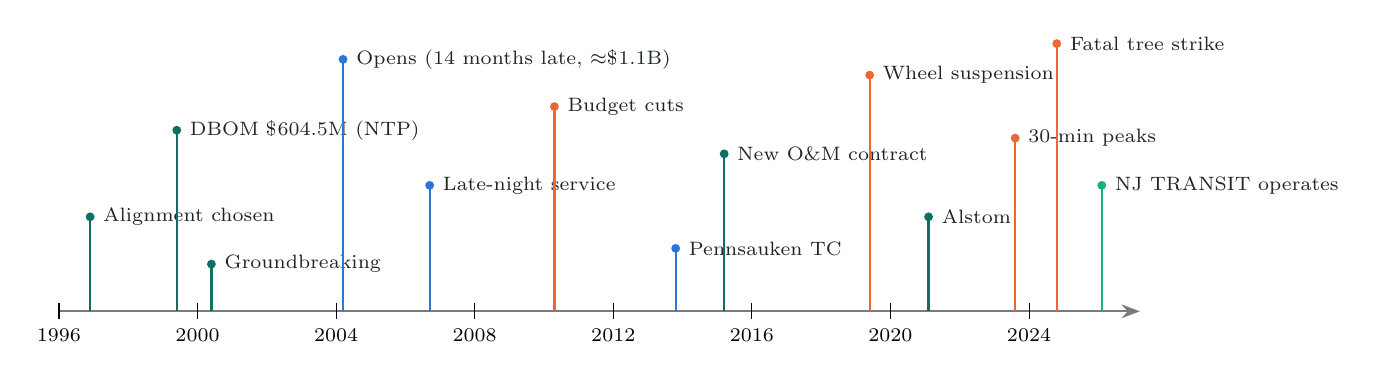
\begin{tikzpicture}[font=\scriptsize, x=0.44cm]
\draw[thick, ink!60, -{Stealth}] (0,0) -- (31.2,0);
\foreach \y in {1996,2000,2004,2008,2012,2016,2020,2024} { \draw ({\y-1996},0.1)--({\y-1996},-0.1); \node[below] at ({\y-1996},-0.1) {\y}; }
\newcommand\ev[4]{\draw[#4, thick] ({#1-1996},0) -- ({#1-1996},#2); \fill[#4] ({#1-1996},#2) circle (1.6pt); \node[anchor=west, text=ink, align=left] at ({#1-1996+0.1},#2) {#3};}
\ev{1996.9}{1.2}{Alignment chosen}{acc}
\ev{1999.4}{2.3}{DBOM \$604.5M (NTP)}{acc}
\ev{2000.4}{0.6}{Groundbreaking}{acc}
\ev{2004.2}{3.2}{Opens (14 months late, $\approx$\$1.1B)}{nb}
\ev{2006.7}{1.6}{Late-night service}{nb}
\ev{2010.3}{2.6}{Budget cuts}{sb}
\ev{2013.8}{0.8}{Pennsauken TC}{nb}
\ev{2015.2}{2.0}{New O\&M contract}{acc}
\ev{2019.4}{3.0}{Wheel suspension}{sb}
\ev{2021.1}{1.2}{Alstom}{acc}
\ev{2023.6}{2.2}{30-min peaks}{sb}
\ev{2024.8}{3.4}{Fatal tree strike}{sb}
\ev{2026.1}{1.6}{NJ TRANSIT operates}{gr}
\end{tikzpicture}
\caption{River LINE timeline. Blue: service milestones; orange: setbacks; teal: contracts; green: takeover. Sources in Section~\ref{sec:history} and Table~\ref{tab:timeline}.}\label{fig:timeline}
\end{figure}

{\small
\begin{longtable}{@{}p{2.1cm}p{9.6cm}p{2.9cm}@{}}
\caption{Dated events and sources.}\label{tab:timeline}\\
\toprule Date & Event & Source \\ \midrule \endfirsthead
\toprule Date & Event & Source \\ \midrule \endhead
1996-11 & NJ TRANSIT board picks the Bordentown Secondary alignment & \flag{W} \citep{wiki_riverline} \\
1998-12 & Bechtel/Adtranz team low bidder for DBOM & \citep{bechtel1998} \\
1999-05-12 & Notice to proceed; \$604.5M DBOM (\$453.3M D/B + \$151.2M O\&M, 13 years) & \citep{njdot2000groundbreaking} \\
1999-08-23 & FRA waiver petition (temporal separation) published & \citep{fr1999waiver} \\
2000-05-08 & Groundbreaking in Camden & \citep{njdot2000groundbreaking} \\
2002-08 & First Stadler GTW car arrives & \citep{pesky2025} \\
2003-11-12 & Opening announced for Feb 15, 2004 (missed) & \citep{njt2003debut} \\
2004-03-14 & Public opening & \citep{camdenhistory2004} \\
2004-06 & 15-minute peak service & \citep{njt2004fifteen} \\
2006-09 & Late-night service and \$1.3M signal work announced; earlier and later trips & \citep{njt2006latenight,njt2006earlier} \\
2008-03-31 & Record weekday ridership, 7{,}600 & \citep{njt2008ridership} \\
2010-03-05 & Service cuts proposed amid \$300M deficit (effective May 1) & \citep{njt2010fare} \\
2013-10-14 & Pennsauken Transit Center opens (\$40M) & \citep{inquirer2013pennsauken} \\
2014-10-01 & Bombardier O\&M contract, about \$296M, effective 2015-03-14 & \citep{masstransit2014bombardier} \\
2019-06-07 & Service suspended for wheel inspections, restored 06-10 & \citep{cbs2019wheels} \\
2021-01-29 & Alstom completes purchase of Bombardier & \citep{alstom2021} \\
2023-08 & 80.4\% on time; 30-minute peaks & \citep{inquirer2023} \\
2024-07-25 & Sen.~Singleton asks for legislative hearings & \citep{insidernj2024} \\
2024-08-12 & Interim 30-minute schedule; buses at six stations & \citep{njt2024interim} \\
2024-10-14 & Fatal collision with fallen tree near Florence & \citep{ntsb2025} \\
2024-10-22 & First River LINE public safety meeting, Palmyra & \citep{cbs2024meeting} \\
2025-09-03 & NJ TRANSIT--Alstom joint statement on takeover & \citep{njt2025alstom} \\
2025-11-13 & Public meeting: fleet to be rebuilt or replaced in 5--7 years & \citep{centraljersey2025} \\
2025-12-12 & Alstom lays off 121 staff & \citep{patch2025layoffs} \\
2026-01-09 & First rehabilitated car; fleet-replacement RFP in development & \citep{njt2026rehab} \\
2025-11-12 & Board creates NJ TRANSIT Southern Light Rail, Inc. (item 2511-51) & \citep{njt2025board} \\
2026-02-14 & NJ TRANSIT operates and maintains the line (Kinkisharyo for vehicles) & \citep{ols2027njt,njt2025board} \\
2026-05-06 & Petition to extend FRA shared-use waiver & \citep{fr2026waiver} \\
\bottomrule
\end{longtable}}

\paragraph{When was the system last updated?} There has been no full overhaul since opening. The most recent work is:
\begin{itemize}
\item the 2026 interior rehabilitation of 14 of the 20 cars, with engine overhauls \citep{njt2026rehab};
\item real-time arrival displays at every station, installed in 2025--26 \citep{njt2026rehab};
\item 17 new auxiliary power units and \$19 million of infrastructure, signage, track, signal, parts, and lighting work reported at the November 2025 public meeting \citep{centraljersey2025};
\item removal of 111 hazard trees after the 2024 collision \citep{ntsb2025}.
\end{itemize}
A mid-life overhaul of the 20 cars appears in the regional capital program (NJTPA TIP project T550) \citep{njtpa_tip}.

%======================================================================
\section{Riders}\label{sec:riders}
\subsection{Who rides}
The only River LINE-specific on-board survey we found was done by DVRPC on November 17, 2010, and yielded 1{,}265 usable responses \citep{dvrpc2013}. Its main findings:
\begin{itemize}
\item \textbf{Trip purpose.} 63\% of trips were to work and 10\% to college; 79\% of respondents rode four or more days a week.
\item \textbf{Riders.} Mean age was 42; 40\% were African American, 40\% white, and 13\% Hispanic.
\item \textbf{Income and cars.} Mean household income was \$55{,}749, and 21\% of households earned under \$25{,}000. 21\% had no vehicle.
\item \textbf{Getting to the train.} 35\% drove and parked, 34\% walked, and 16\% transferred from other transit (Figure~\ref{fig:dvrpc}).
\item \textbf{Getting from the train.} 47\% walked and 38\% transferred, including 14\% to PATCO and 10\% to NJ TRANSIT buses.
\item \textbf{Where trips go.} The biggest destinations were Trenton (21\%), Camden (18\%), and Philadelphia (16\%).
\end{itemize}
A 2008 Rutgers household survey near the line (800 households) found that 61\% of riders walked to stations \citep{chatman2010}.

The NJTOD newsletter's figures of ``69 percent walk'' and ``46 percent have no car'' \citep{njtod2026} come from APTA's national survey of all transit riders \citep{apta2017who}. They are not River LINE-specific and should not be quoted as such.

\subsection{How satisfied they are}
\begin{itemize}
\item \textbf{2010.} In the DVRPC survey, 68\% of riders rated the River LINE 8 or higher out of 10 overall. The share giving a perfect 10 ranged from 40\% for fares to 21\% for customer communication, the lowest-rated attribute. Personal security and connections also rated low (Figure~\ref{fig:dvrpc}) \citep{dvrpc2013}.
\item \textbf{2011--2012.} NJ TRANSIT's first published satisfaction surveys scored light rail as a whole 6.5 (2011) and 6.9 (2012). The system overall scored 5.2 and 5.8 \citep{njt2011survey,njt2012survey}.
\item \textbf{2019--2025, by line.} NJ TRANSIT's wave reports \citep{njtcss2022fall,njtcss2023fall,njtcss2024fall,njtcss2025fall} show the River LINE's overall score by wave (Table~\ref{tab:css}, Figure~\ref{fig:css}). It was the lowest of the three light rail lines in every wave from Spring 2022 to Fall 2025. It declined steadily from 6.6 to 5.9, then rose to 6.8 in Fall 2025. NJ TRANSIT attributes the rise to the September 2025 takeover announcement, fewer cancellations, and faster service alerts \citep{njtcss2025fall}. Our Fall 2024 figure of 6.1 from the press \citep{njcom2025survey} matches the report.
\end{itemize}

\begin{table}[ht]\centering\small
\begin{tabular}{@{}lcccccccccc@{}}
\toprule
& \multicolumn{2}{c}{2019} & \multicolumn{2}{c}{2022} & \multicolumn{2}{c}{2023} & \multicolumn{2}{c}{2024} & \multicolumn{2}{c}{2025} \\
Line & Spr & Fall & Spr & Fall & Spr & Fall & Spr & Fall & Spr & Fall \\
\midrule
River LINE & 6.3 & 6.6 & 6.6 & 6.4 & 6.4 & 6.2 & 6.1 & 6.1 & 5.9 & \textbf{6.8} \\
Hudson--Bergen & -- & -- & 6.8 & 6.8 & 6.7 & 6.9 & 6.6 & 6.5 & 6.4 & 7.0 \\
Newark Light Rail & -- & -- & 7.1 & 6.7 & 7.1 & 7.1 & 7.3 & 6.9 & 6.8 & 7.0 \\
\bottomrule
\end{tabular}
\caption{Overall satisfaction (0--10) by light rail line, read from the charts in NJ TRANSIT's survey reports \citep{njtcss2022fall,njtcss2023fall,njtcss2024fall,njtcss2025fall}. No surveys were run in 2020--21.}\label{tab:css}
\end{table}
\begin{figure}[ht]\centering
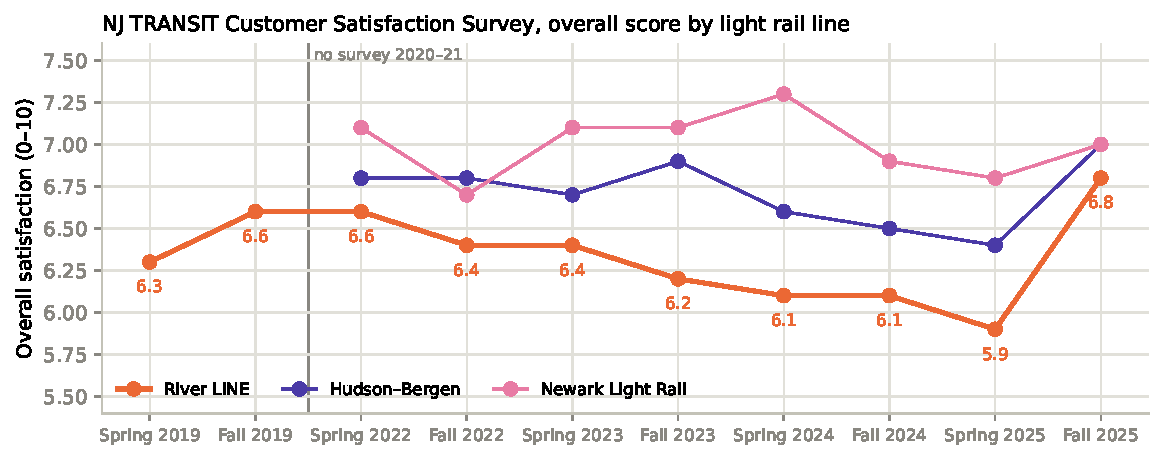
\includegraphics[width=\textwidth]{fig_ctx_satisfaction.pdf}
\caption{Overall satisfaction by light rail line \citep{njtcss2022fall,njtcss2023fall,njtcss2024fall,njtcss2025fall}.}\label{fig:css}
\end{figure}

\paragraph{Which attributes matter most to River LINE riders.} The reports list each line's ten most important attributes and how they score:
\begin{itemize}
\item \textbf{Most important.} The weekday AM peak schedule, safety, security, and on-time performance at the boarding station rank highest.
\item \textbf{Fall 2023} (mean scores). The lowest were cleanliness on board (4.71), security (5.16), seating availability (5.69), and safety (5.87) \citep{njtcss2023fall}.
\item \textbf{Fall 2024} (share scoring 5 or more). Cleanliness on board 53\%, security 59\%, seating 73\%, on time 73\%, AM peak schedule 78\%, safety 82\% \citep{njtcss2024fall}.
\item \textbf{Fall 2025.} Every top-ten attribute improved on Spring 2025. On time at boarding rose from about 67\% to about 83\%, and ``handling of service disruptions'' from about 53\% to about 63\%. These values are read from bars without printed labels \citep{njtcss2025fall}.
\end{itemize}
Security, cleanliness, and the handling of disruptions are the persistent weak points. Schedule reliability is the attribute that moved most after the takeover.

\begin{figure}[ht]\centering
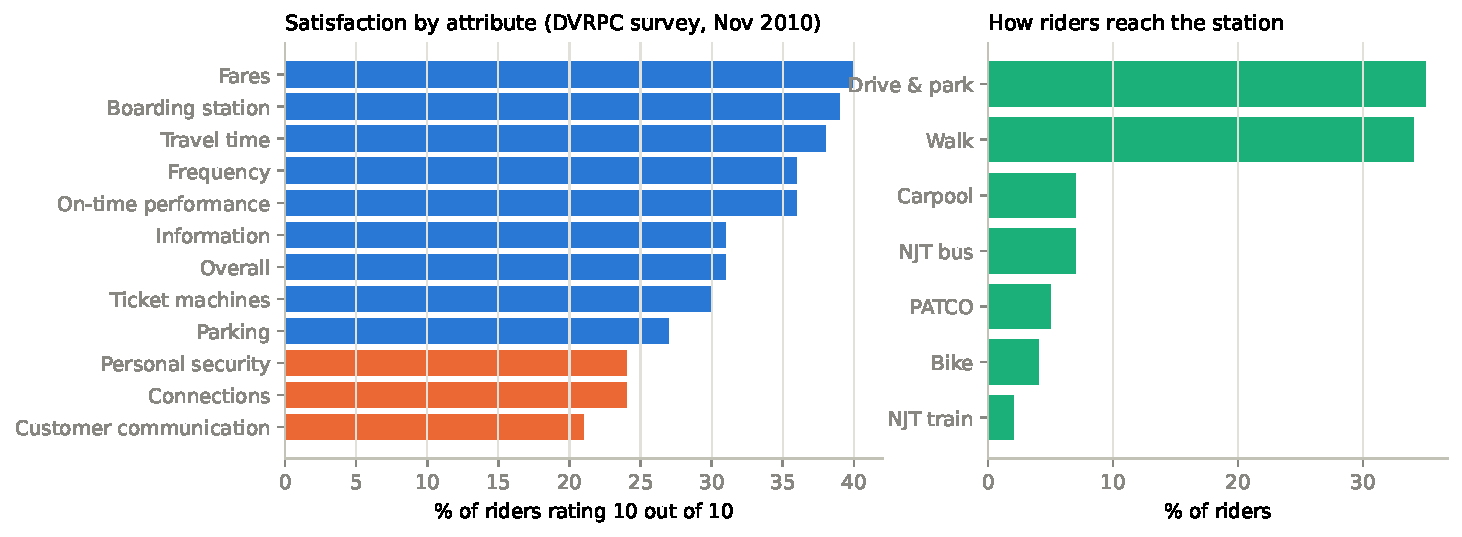
\includegraphics[width=\textwidth]{fig_ctx_dvrpc.pdf}
\caption{Left: share of riders rating each attribute 10 out of 10. Right: how riders reached their boarding station. DVRPC on-board survey, November 2010 \citep{dvrpc2013}.}\label{fig:dvrpc}
\end{figure}

\subsection{What riders and officials have said}
\begin{itemize}
\item \textbf{July 2024.} State Senator Troy Singleton (Burlington) called the service ``simply inexcusable'' and asked for Senate Transportation Committee hearings. It was the third straight summer of disruptions \citep{insidernj2024}.
\item \textbf{October 2024.} At a meeting in Palmyra after the fatal crash and an August pedestrian death, residents raised delays, cleanliness, train speeds, and crossing gates. NJ TRANSIT committed \$19 million over five years to fleet upgrades, plus fencing and school outreach \citep{cbs2024meeting}.
\item \textbf{November 2025.} At a second Palmyra meeting, riders raised fights, loud music, and panhandling at stations, and asked for fare enforcement. NJ TRANSIT reported that delays and cancellations were 22\% lower than in 2024 \citep{centraljersey2025}.
\item \textbf{Constituent complaints} forwarded by Senator Singleton cited ``inconvenient cancellations and delays, little to no communication, dirty and unkempt stations and trains'' \citep{singleton2025}.
\end{itemize}

\subsection{What the literature says riders value}
Frequency and travel time are the attributes riders rank highest \citep{transitcenter2016}. Unreliability makes riders leave earlier, switch routes, or switch modes \citep{carrel2013}. Reliability measurably affects ridership \citep{chakrabarti2015}. Riders weigh waiting and lateness well above time on board \citep{wardman2004}, and reviews put the value of reliability at roughly 0.5--1.5 times the value of travel time \citep{carrion2012}.

Commute experience matters for well-being:
\begin{itemize}
\item Longer and less predictable commutes lower life satisfaction \citep{stutzer2008}.
\item Commute satisfaction differs by mode and is driven by trip duration and reliability \citep{stlouis2014}.
\item Travel affects well-being directly and through the activities it makes possible \citep{ettema2010,devos2013}.
\end{itemize}
Real-time information, which the River LINE now has at every station, has been linked to modest ridership gains \citep{brakewood2015}.

%======================================================================
\section{Ridership and performance}\label{sec:ridership}
\subsection{Ridership}
Figure~\ref{fig:annual} shows NTD trips by calendar year and Figure~\ref{fig:monthly} the months since 2023. Before the pandemic the line carried 2.65--2.90 million trips a year. That is well above the opening projection of about 6{,}000 weekday riders \citep{reason2004}: 9{,}014 per weekday in FY2014 \flag{W}.

Ridership fell to 1.51 million in 2021, recovered only to 1.78--1.81 million in 2022--24, and fell again to 1.63 million in 2025. That is 61\% of 2019 on the NTD numbers (NJTOD reports 59\%) \citep{njtod2026}. OLS reports the same pattern by fiscal year: 1.71, 1.76, and 1.86 million trips in FY2022--24 and 1.73 million projected for FY2025 \citep{ols2026njt}.

Since the takeover, June 2026 had 167{,}158 trips against 136{,}609 in June 2025 (+22\%), and July had 173{,}347 against 155{,}017 (+12\%) \citep{ntd_monthly}.

\paragraph{A figure to avoid.} Wikipedia's 8{,}633 average weekday riders for 2024 \flag{W} is inconsistent with 1.8 million annual trips. It matches pre-pandemic levels, so it is probably a stale figure. The NTD numbers should be used instead.

\begin{figure}[ht]\centering
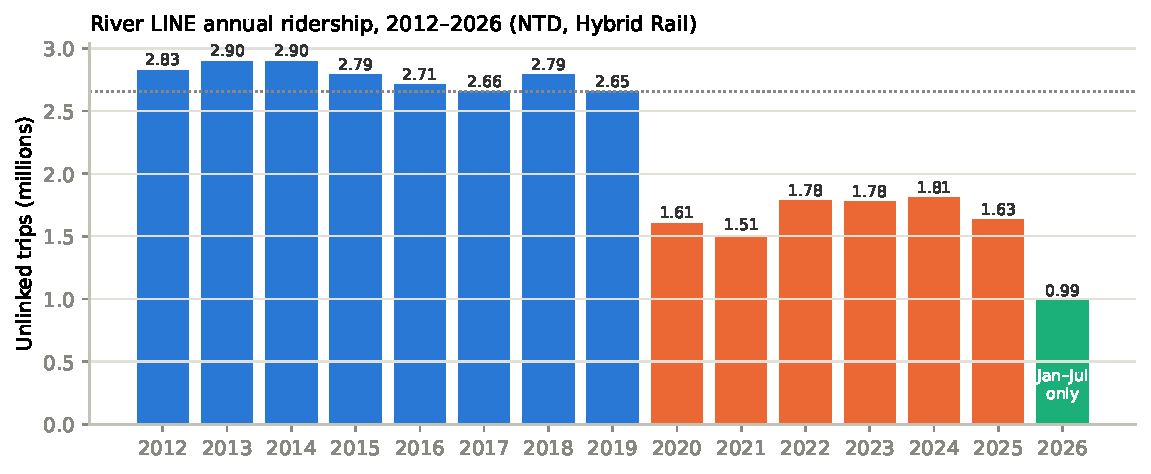
\includegraphics[width=\textwidth]{fig_ctx_ridership_annual.pdf}
\caption{Annual unlinked trips, NTD Monthly Module, NJ TRANSIT (ID 20080), Hybrid Rail \citep{ntd_monthly}. Blue: before 2020; orange: 2020--25; green: January--July 2026 only. Dotted: 2019.}\label{fig:annual}
\end{figure}
\begin{figure}[ht]\centering
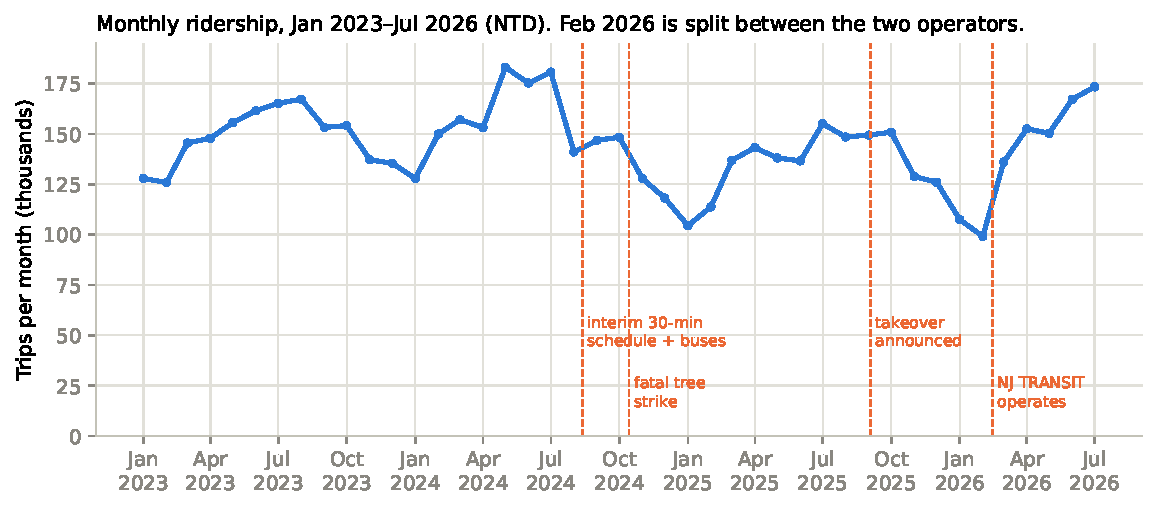
\includegraphics[width=\textwidth]{fig_ctx_ridership_monthly.pdf}
\caption{Monthly trips, January 2023--July 2026 \citep{ntd_monthly}, with events from \citep{njt2024interim,ntsb2025,njt2025alstom,ols2027njt}.}\label{fig:monthly}
\end{figure}

\subsection{Reliability and on-time performance}
Figure~\ref{fig:perf} collects the reported on-time rates and failure intervals. Definitions vary by source, so the bars are not strictly comparable.
\begin{itemize}
\item \textbf{Before the takeover:}
  \begin{itemize}
  \item August 2023: 80.4\% on time \citep{inquirer2023}.
  \item 2024--25: about 87\% of scheduled service on time, with worst days of 45\% (summer 2024) and 56\% (summer 2025) \citep{ols2027njt}.
  \item July 2025: 82.3\%, against a 97\% goal \citep{news12_2025}.
  \item Calendar 2025: 84\%, against 97\% on Hudson--Bergen and 99\% on Newark Light Rail \citep{njtod2026}.
  \end{itemize}
\item \textbf{After the takeover:} ``above 93 percent'' \citep{ols2027njt}. NJ TRANSIT's public dashboard showed the River LINE at 86.2\%, Newark Light Rail at 99.1\%, and Hudson--Bergen at 96.5\% when printed on September 28, 2026. The period behind those bars is not stated on the printout \citep{njt_otpdash}. The downloadable on-time file covers all light rail combined, not the River LINE alone \citep{njt_otp}.
\item \textbf{Miles between failures:} 22{,}337 in 2022 and 4{,}192 in 2024 \citep{roinj2025}. NJ TRANSIT's own monthly series (Figure~\ref{fig:mdbf}) \citep{njt_mdbf}, which moves smoothly and so appears to be a rolling average, shows:
  \begin{itemize}
  \item about 9{,}000 miles in 2017, drifting down to about 5{,}600 in late 2019;
  \item a rise to about 22{,}000 in 2021--22, when service and ridership were reduced;
  \item a collapse to 4{,}000--4{,}300 through 2024 and a low of 2{,}377 in September 2025;
  \item recovery to 3{,}600--3{,}800 in June--August 2026 under NJ TRANSIT.
  \end{itemize}
  The River LINE has been the least reliable of the three light rail lines since mid-2024. NTD failure counts for the River LINE (Table~\ref{tab:ntdfail}) show the same trend on a different definition: car-miles per major mechanical failure fell from 6{,}537 (FY2022) to 3{,}734 (FY2024), and total failures more than doubled, from 192 to 435 \citep{ntd_breakdowns2224}.
\item \textbf{NTD service data:} the maximum number of vehicles in service fell from 16 through January 2026 to 8--12 after the takeover. Revenue miles fell from 1.23 million (2019) to 0.90 million (2025) \citep{ntd_monthly}.
\end{itemize}
The takeover-era service therefore runs fewer trains more reliably, and ridership has risen with it.

\begin{table}[ht]\centering\small
\begin{tabular}{@{}lrrrrr@{}}
\toprule
NTD report year & Major failures & Other failures & Car-miles & Car-miles per major failure & Car-miles per failure \\
\midrule
2022 & 181 & 11 & 1{,}183{,}194 & 6{,}537 & 6{,}162 \\
2023 & 244 & 19 & 1{,}052{,}435 & 4{,}313 & 4{,}002 \\
2024 & 267 & 168 & 997{,}015 & 3{,}734 & 2{,}292 \\
\bottomrule
\end{tabular}
\caption{River LINE mechanical failures, NTD 2022--2024 Breakdowns (Hybrid Rail, purchased transportation) \citep{ntd_breakdowns2224}. A major failure prevents the vehicle from completing or starting its trip.}\label{tab:ntdfail}
\end{table}

\begin{figure}[ht]\centering
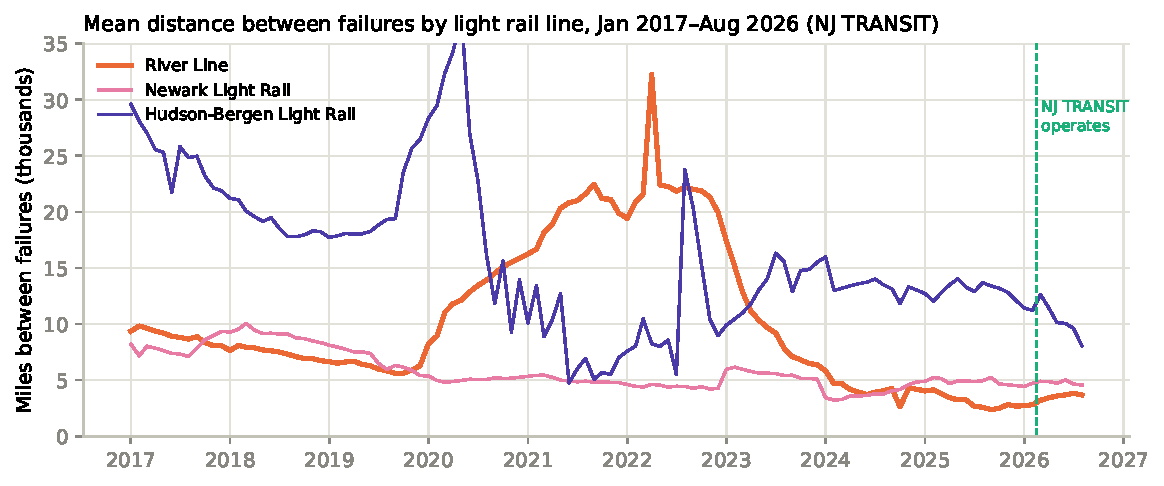
\includegraphics[width=\textwidth]{fig_ctx_mdbf.pdf}
\caption{Mean distance between failures by light rail line, January 2017--August 2026 \citep{njt_mdbf}.}\label{fig:mdbf}
\end{figure}
\begin{figure}[ht]\centering
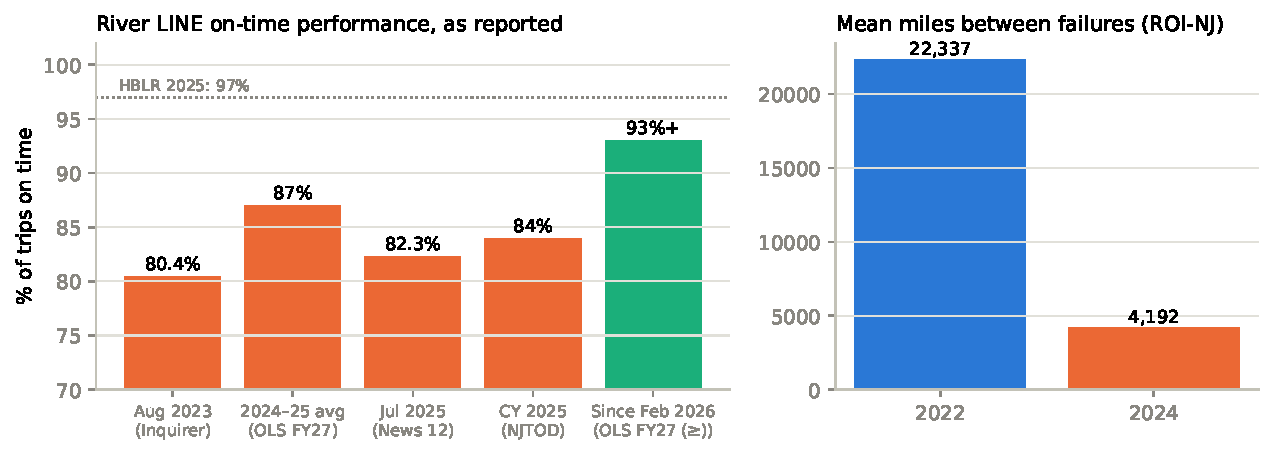
\includegraphics[width=\textwidth]{fig_ctx_performance.pdf}
\caption{Left: on-time performance as reported by each source \citep{inquirer2023,ols2027njt,news12_2025,njtod2026}; definitions differ. Right: mean miles between failures \citep{roinj2025}.}\label{fig:perf}
\end{figure}

%======================================================================
\section{Money}\label{sec:money}
\subsection{Capital}
\begin{itemize}
\item \textbf{Construction:} over \$1 billion, about \$1.1 billion, all state funds \citep{camdenhistory2004,njtod2026,chatman2010}.
\item \textbf{Original DBOM:} \$604.5 million, of which \$453.3 million was design--build \citep{njdot2000groundbreaking}. Reason Foundation put the early estimate at \$450 million \citep{reason2004}.
\item \textbf{Later capital:}
  \begin{itemize}
  \item Pennsauken Transit Center, \$40 million, mostly federal stimulus \citep{inquirer2013pennsauken};
  \item \$1.3 million of signal work in 2006 \citep{njt2006latenight};
  \item \$19 million committed in 2024 for fleet upgrades \citep{cbs2024meeting};
  \item \$19 million invested in infrastructure by November 2025 \citep{centraljersey2025}.
  \end{itemize}
\item \textbf{Regional capital programs:}
  \begin{itemize}
  \item DVRPC TIP project T95, Light Rail Infrastructure Improvements, explicitly includes ``River Line capital asset replacement.'' It carries \$4.27 million of state money a year in FY2024--27, shared with Newark and Hudson--Bergen \citep{dvrpc_t95}.
  \item NJTPA TIP project T550 includes a mid-life overhaul of the 20 River LINE cars: about \$20 million for 2026--29 and \$20 million more for 2030--35. The line also carries other light rail items \citep{njtpa_tip}.
  \end{itemize}
\item \textbf{Fleet replacement:} no cost or award has been published.
\end{itemize}

\subsection{Operations}
\begin{itemize}
\item \textbf{Contract payments.} The 1999 DBOM included \$151.2 million for operations and maintenance \citep{njdot2000groundbreaking}. The 2015 contract was about \$296 million over 15 years \citep{masstransit2014bombardier}. By FY2025, monthly payments were \$2.26 million, escalating about 2.83\% a year \citep{ols2026njt}.
\item \textbf{Cost of the contract and of the takeover.} The FY2025 contract cost was \$37.5 million. Running the line in-house costs \$40.6 million, \$3.1 million more \citep{ols2027njt}.
\item \textbf{Staffing.} The FY2027 budget exhibit in the April 2026 board agenda lists ``River LINE insourcing: 94 FTE, \$3.9m'' among new service needs \citep{njt2026board}. The operating company is a new subsidiary, NJ TRANSIT Southern Light Rail, Inc., created by the board in November 2025 \citep{njt2025board}.
\item \textbf{Ten-year cost history} (Figure~\ref{fig:ts21}) \citep{ntd_ts21}:
  \begin{itemize}
  \item Operating cost ranged from \$30.8 million to \$37.0 million a year over 2015--2024.
  \item Cost per revenue hour rose from about \$700 (2015, 2019) to \$952 (2024) as revenue hours fell from 52{,}000 to 38{,}000.
  \item Vehicle maintenance spending nearly doubled, from \$5.1 million (2019) to \$9.3 million (2024).
  \item Farebox recovery fell from about 7\% before 2020 to 2--3\% since 2021.
  \end{itemize}
  The 2019 NTD agency profile puts the line at \$705 per revenue hour and \$12.61 per trip \citep{ntd_profile2019}.
\item \textbf{NTD unit costs} (Table~\ref{tab:ntd}, Figure~\ref{fig:costs}). Operating cost was \$36.4 million in FY2024: \$952 per vehicle revenue hour and \$19.57 per trip. Fare revenue was \$0.86 million, or \$0.46 per trip \citep{ntd_metrics2224}.
\item \textbf{Farebox recovery.} OLS reports 3.5\%, 4.2\%, 2.6\%, and 2.7\% for FY2022--25 \citep{ols2026njt}. Fare revenue per trip is far below the \$1.90 fare \citep{njt_fares}, probably because of reduced fares, passes, and transfers.
\item \textbf{NJ TRANSIT as a whole.} The operating budget was \$3.16 billion in FY2026 and \$3.5 billion in FY2027 \citep{njt_fy26budget,njt_fy27budget}. The River LINE's roughly \$40 million is about 1\% of it.
\end{itemize}

\begin{table}[ht]\centering\small
\begin{tabular}{@{}lrrr@{}}
\toprule
NTD report year (fiscal) & 2022 & 2023 & 2024 \\
\midrule
Operating expense (\$M) & 34.86 & 37.02 & 36.38 \\
Fare revenue (\$M) & 1.03 & 0.98 & 0.86 \\
Unlinked trips (M) & 1.71 & 1.76 & 1.86 \\
Vehicle revenue hours (000) & 45.4 & 41.0 & 38.2 \\
Vehicle revenue miles (M) & 1.16 & 1.02 & 0.95 \\
Passenger miles (M) & 25.0 & 26.1 & 27.0 \\
Cost per revenue hour (\$) & 769 & 904 & 952 \\
Cost per trip (\$) & 20.36 & 21.06 & 19.57 \\
Fare per trip (\$) & 0.60 & 0.56 & 0.46 \\
\bottomrule
\end{tabular}
\caption{River LINE (Hybrid Rail, purchased transportation) in the NTD 2022--2024 metrics \citep{ntd_metrics2224}. The average trip is about 14.5 miles.}\label{tab:ntd}
\end{table}
\begin{figure}[ht]\centering
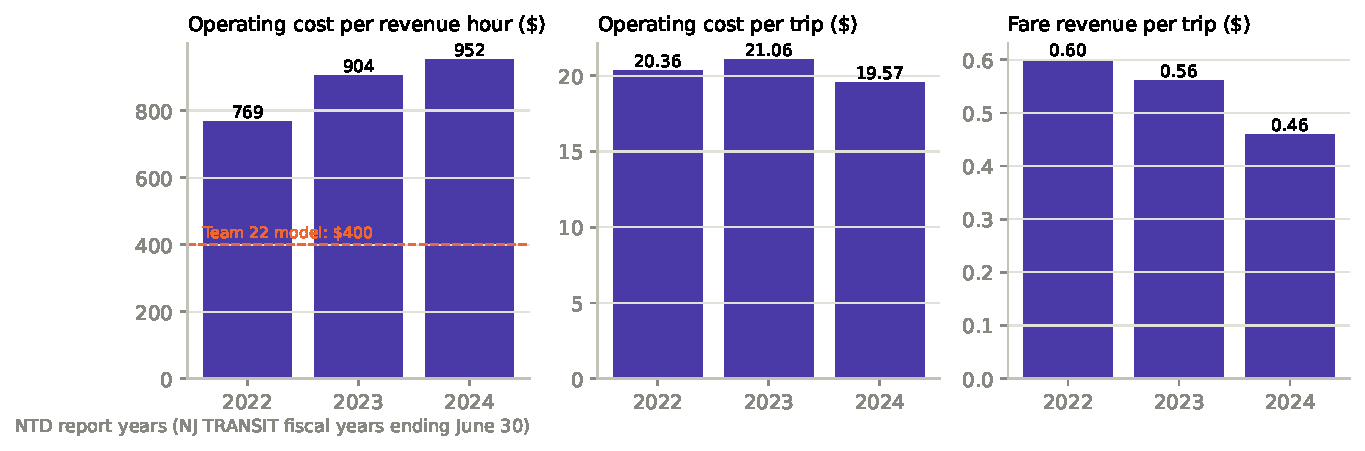
\includegraphics[width=\textwidth]{fig_ctx_costs.pdf}
\caption{NTD unit costs \citep{ntd_metrics2224}. Dashed line: the \$400 per train-hour our schedule model assumed.}\label{fig:costs}
\end{figure}
\begin{figure}[ht]\centering
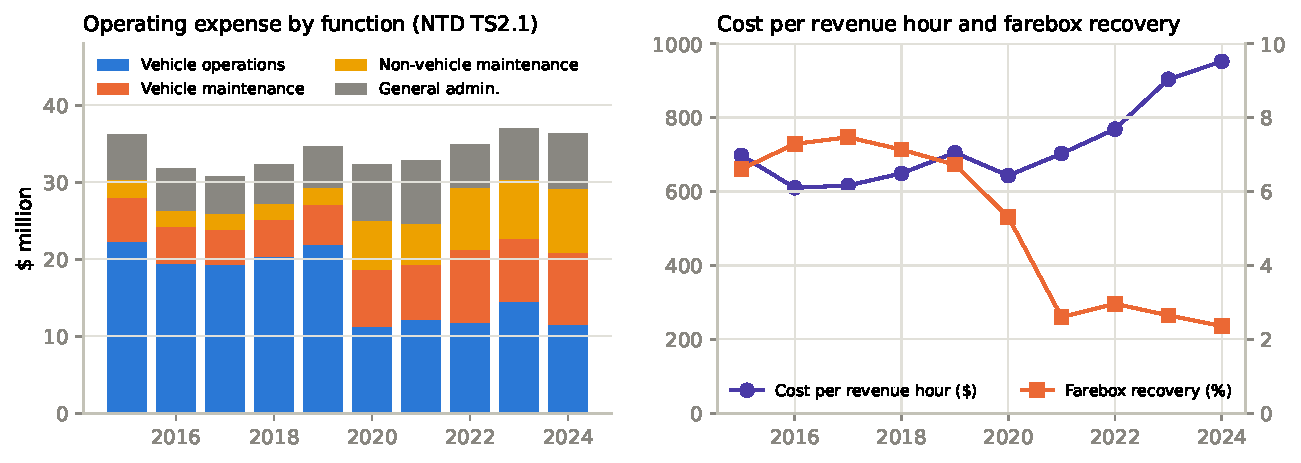
\includegraphics[width=\textwidth]{fig_ctx_ts21.pdf}
\caption{River LINE operating expense by function, cost per revenue hour, and farebox recovery, NTD report years 2015--2024 \citep{ntd_ts21}.}\label{fig:ts21}
\end{figure}

%======================================================================
\section{Effects on the towns and on people}\label{sec:impacts}
\subsection{Studies of the River LINE}
The main evaluation is a Rutgers study for NJDOT \citep{chatman2010}. It combined interviews, land-use and zoning review, surveys of 800 households and of firms, and real-estate data. It found ``modest and mixed'' economic development effects:
\begin{itemize}
\item \textbf{Ridership near the line.} 24\% of households within half a mile of a station had ridden in the past month, against 5\% farther away.
\item \textbf{Where people live.} Only 4\% named the line as a reason for where they lived, yet 72\% said it had improved quality of life.
\item \textbf{Firms.} The share of workers commuting by River LINE fell from 8.6\% within one-eighth mile of a station to 0.4\% beyond half a mile.
\item \textbf{Local change.} Growth in building permits did not accelerate after 2004, and zoning and redevelopment changes were ``relatively modest.''
\end{itemize}

The peer-reviewed companion found the net effect on owner-occupied home values neutral to slightly negative \citep{chatman2012}. Smaller homes and lower-income areas near stations gained value, possibly at the expense of homes farther away. Homes near high-ridership stations did worse, and homes near stations with parking did better.

Later work by NJTOD and the Voorhees Transportation Center \citep{njtod2026} explains part of the gap:
\begin{itemize}
\item Only 35\% of land within station areas is in transit-supportive use, against 60--65\% on Hudson--Bergen and Newark Light Rail.
\item Only 7 of 21 stations are in traditional downtowns.
\item The Pennsauken Transit Center has 121 River LINE boardings against 570 projected.
\end{itemize}
The same newsletter lists recent transit-oriented projects:
\begin{itemize}
\item The Mill at Riverside (190 units, 2026);
\item Pearl Pointe in Burlington (184 units, 2021);
\item Oliver Station in Camden (47 affordable senior units);
\item Parkside Place in Camden (30 affordable units with retail, supported by an \$18 million state grant).
\end{itemize}
Riverside (2001) and Burlington (2007) are designated Transit Villages. A Bordentown waterfront infill station and housing were proposed in 2010 \citep{njtod2010bordentown}.

\subsection{What the broader literature says}
\begin{itemize}
\item \textbf{Property values.} In a meta-analysis, homes within a quarter mile of a rail station sell for about 4\% more and commercial property for about 16\% more, with larger effects for commuter rail than light rail \citep{debrezion2007}. Effects vary widely by land use, rail type, and region \citep{mohammad2013}. Buffalo's light rail showed a modest premium near stations \citep{hess2007}.
\item \textbf{Jobs and the economy.} When post-Sandy repairs removed R train service in Brooklyn, unemployment near its stations rose \citep{tyndall2017}. APTA's national estimate is about 17{,}900 jobs per \$1 billion of transit spending \citep{apta2020econ}, but that is an input--output estimate, not a causal one. Evidence that transit raises productivity through agglomeration is thin \citep{chatman2011agg}.
\item \textbf{Ridership.} Across 25 North American cities, service supply is the strongest driver of transit ridership \citep{boisjoly2018}. Reliability improvements can be valued like travel-time savings in cost--benefit analysis \citep{vanoort2016}.
\item \textbf{Well-being.} See Section~\ref{sec:riders}; commuting stress lowers life satisfaction \citep{stutzer2008,stlouis2014,ettema2010,devos2013}.
\end{itemize}

For the River LINE this suggests that reliable, frequent service matters to the people who already depend on it. The 21\% without a car and the 63\% commuting to work \citep{dvrpc2013} bear the cost of every cancelled train. Development benefits, by contrast, depend mostly on land use near stations, which municipalities control, not on the timetable.

%======================================================================
\section{What went wrong}\label{sec:wrong}
\begin{table}[ht]\centering\small
\begin{tabularx}{\textwidth}{@{}p{3.6cm}L p{2.5cm}@{}}
\toprule
Problem & What happened & Sources \\
\midrule
Cost and schedule at opening & About \$1.1B against early estimates of about \$450M; opened 14 months late & \citep{camdenhistory2004,reason2004} \\
Low early ridership & About 1{,}500 per day in the first weeks against about 6{,}000 projected & \citep{reason2004} \\
Budget cuts & 2010: fewer two-car trains; late-night service only on event nights & \citep{njt2010fare} \\
One-off fleet & Custom cars with scarce parts; engines, HVAC, and auxiliary power units failing; engine rebuilds stalled (1 of 18 done by October 2023) & \citep{inquirer2023,singleton2025,njt2024interim} \\
Reliability collapse & 22{,}337 to 4{,}192 miles between failures (2022--24); worst days 45\% and 56\% on time & \citep{roinj2025,ols2027njt} \\
Service cuts & 30-minute peaks in 2023; interim 30-minute schedule and buses in 2024 & \citep{inquirer2023,njt2024interim} \\
Safety & Fatal tree strike, October 2024 (four earlier tree strikes in 18 months); pedestrian deaths & \citep{ntsb2025,singleton2025} \\
Wheel defect & Line shut June 7--10, 2019 & \citep{cbs2019wheels} \\
Communication and stations & Lowest-rated attribute in 2010; recurring complaints about communication, cleanliness, and security & \citep{dvrpc2013,singleton2025,centraljersey2025} \\
Contracting model & Contract scope did not cover the investment the aging system needed; ended by mutual agreement & \citep{njt2025alstom,railwaygazette2025} \\
Land use & 35\% transit-supportive land; weak development response & \citep{njtod2026,chatman2010} \\
\bottomrule
\end{tabularx}
\caption{What went wrong.}
\end{table}

%======================================================================
\section{What worked}\label{sec:worked}
\begin{itemize}
\item \textbf{Demand beat the forecast.} Before COVID, weekday ridership of about 7{,}600--9{,}000 exceeded the opening projection \citep{njt2008ridership,reason2004}, and FY2009 ridership grew while national transit fell \citep{tstc2011}.
\item \textbf{Riders were once satisfied.} In 2010, 68\% rated the line 8 or better out of 10 \citep{dvrpc2013}.
\item \textbf{Cheaper to build.} Diesel light rail on a freight line under temporal separation avoided electrification and a new right of way \citep{fr1999waiver}.
\item \textbf{Service expansions.} Late-night service in 2006 \citep{njt2006latenight}, event service to the waterfront, and the 2013 connection to the Atlantic City Line \citep{inquirer2013pennsauken}.
\item \textbf{The 2026 takeover.} On-time performance above 93\% \citep{ols2027njt}, ridership up 12--22\% year over year \citep{ntd_monthly}, delays and cancellations 22\% lower in 2025 than 2024 \citep{centraljersey2025}, real-time information at every station, and rehabilitated cars \citep{njt2026rehab}.
\item \textbf{Community engagement.} Public meetings in Palmyra in 2024 and 2025 with NJ TRANSIT leadership \citep{cbs2024meeting,centraljersey2025}.
\item \textbf{Housing near stations.} The projects in Riverside, Burlington, and Camden \citep{njtod2026}.
\end{itemize}

%======================================================================
\section{Peer systems with the same trains}\label{sec:peers}
Only three U.S. passenger operators run Stadler GTW diesel units: NJ TRANSIT (20 cars), CapMetro in Austin (10), and DCTA in Denton, Texas (11). San Diego County's Sprinter uses a different Siemens train but is a useful warning.

\begin{table}[ht]\centering\small
\begin{tabularx}{\textwidth}{@{}p{2.6cm}p{2.5cm}L p{2.4cm}@{}}
\toprule
System & Fleet & Experience & Sources \\
\midrule
CapMetro Rail (Austin) & 10 GTW (2007, 2017) & A December 2025 internal audit found many parts could no longer be obtained easily. A September 2026 agreement puts an on-site Stadler team in place for obsolescence and parts support, 2027--2032. & \citep{capmetro2026stadler,railwaysupply2026,capmetro_wiki} \\
DCTA A-train (Denton) & 11 GTW (2011--12), \$73.7M order & Stadler has maintained the fleet under a fixed-price contract since 2020. No public reliability crisis found. & \citep{dcta2009,dcta2020} \\
NCTD Sprinter (San Diego County) & 12 Siemens Desiro (2006) & Shut March--May 2013 over brake wear. By 2025 only 5 of 12 were serviceable. Replacement estimated at \$351M for vehicles plus \$542M for infrastructure. A Buy America waiver for original-manufacturer parts was proposed in June 2026. & \citep{trains2025sprinter,fr2026nctd} \\
\bottomrule
\end{tabularx}
\caption{Peer fleets.}
\end{table}

The lessons for the River LINE:
\begin{enumerate}
\item Small ``boutique'' diesel fleets run into parts obsolescence at around 15--20 years; the River LINE's cars are 22--24 years old.
\item Support contracts with the manufacturer (CapMetro, DCTA) are the usual bridge until new trains arrive.
\item Replacement costs often include large infrastructure work, not just vehicles.
\item Choosing a vehicle other agencies also buy reduces the parts risk.
\end{enumerate}

%======================================================================
\section{What is planned}\label{sec:plans}
\begin{itemize}
\item \textbf{Fleet.} NJ TRANSIT will rebuild or replace the entire fleet within five to seven years (stated November 2025) \citep{centraljersey2025}. A replacement RFP was being developed in January 2026 \citep{njt2026rehab}. The mid-life overhaul is in the TIP \citep{njtpa_tip}, and the 14-car interior rehabilitation is under way \citep{njt2026rehab}.
\item \textbf{Operations.} The operation has been brought in-house through NJ TRANSIT Southern Light Rail, Inc. (94 positions, \$3.9 million) \citep{njt2025board,njt2026board}. The board kept the option to bid operations out to a private company again later \citep{njt2025board}. The FRA shared-use waiver is also to be extended, adding relief under 49~CFR Parts 229 and 238 \citep{fr2026waiver}.
\item \textbf{Glassboro--Camden Line (GCL).} This is an 18-mile, 13-station line from Glassboro to Walter Rand Transportation Center.
  \begin{itemize}
  \item \emph{Status.} The environmental impact statement was completed around 2021 and preliminary engineering began in October 2022 \citep{gcl_timeline,whyy2021gcl}. NJ TRANSIT has been the lead agency since 2024, and the design was 30\% complete in 2025. A 2028 target was stated then \citep{cbs2025gcl}.
  \item \emph{Funding.} In April 2026 the project was estimated at about \$2 billion, with only \$200 million (for design and land) secured \citep{inquirer2026gcl}.
  \item \emph{Plan and link to the River LINE.} Service every 15 minutes, 5\,am--9\,pm, seven days a week, delivered as design--build--operate--maintain, with connection to Trenton via the River LINE \citep{gcl_faq}. A separate \$250 million renovation of Walter Rand is committed \citep{cbs2025gcl}.
  \end{itemize}
\item \textbf{Extensions.} None is funded or in an official plan. Extending to the Trenton State House area (about 0.8 mile) has been discussed \citep{tcnj2017}. A West Trenton extension to SEPTA (about \$658 million) appeared on a 2020 advocacy list \citep{tstc2020}. NJ TRANSIT's 2030 strategic plan and the state's DVRPC-area program list no River LINE extension \citep{njt2030,nj_stip_dvrpc}.
\item \textbf{More capacity.} No project to add sidings or double track was found, so the single track will continue to cap frequency.
\end{itemize}

%======================================================================
\section{What this means for our project}\label{sec:implications}
\begin{enumerate}
\item \textbf{Update the cost parameter.} NTD puts the River LINE at \$952 per vehicle revenue hour in FY2024 \citep{ntd_metrics2224}. Our model assumes \$400 per train-hour. The marginal cost of an extra train-hour is below the average, but probably well above \$400. A higher cost makes the smaller timetables in our playbook more attractive.
\item \textbf{Recalibrate reliability to the takeover.} Our failure parameters reflect 2024 (4{,}192 miles between failures), which NTD's River LINE-specific 3{,}734 car-miles per major failure in FY2024 broadly confirms \citep{ntd_breakdowns2224}. NJ TRANSIT's monthly series shows it got worse: 2{,}400--2{,}800 in September 2025 -- February 2026, recovering to about 3{,}700 by mid-2026 \citep{njt_mdbf}. We should rerun the fleet simulation with the 2025--26 series (roughly 2{,}500 and 3{,}700 miles as ``bad'' and ``current'' cases). Since February 2026 on-time performance is above 93\% with 8--12 trains in service \citep{ols2027njt,ntd_monthly}.
\item \textbf{Fleet renewal changes the question.} With new trains in 5--7 years, the playbook for short days matters most now. The robust timetables (B8 and B7) and the summer plan matter for longer. Timetable work should also feed the replacement specification: how many cars, and with what reliability, are needed for 15-minute service (Section~7 of the main report).
\item \textbf{Communication is part of the product.} The lowest-rated attribute, both in 2010 and in recent complaints, is communication \citep{dvrpc2013,singleton2025}. Publishing the day's timetable by 6\,am and pushing it to the new real-time signs is a direct response.
\item \textbf{Equity.} About one in five riders has no car \citep{dvrpc2013}. Cancellations and bus substitutions should be weighed accordingly, and replacement buses should serve the stations where those riders board.
\item \textbf{Measure the benefits in ridership, not only minutes.} The 12--22\% ridership gain after reliability improved \citep{ntd_monthly}, and the literature linking service to ridership \citep{boisjoly2018,chakrabarti2015}, support adding a ridership response to our cost account.
\item \textbf{Glassboro--Camden Line connection.} If the GCL is built, timed transfers at Walter Rand become a timetable constraint. Our timetable model can take such constraints directly.
\item \textbf{Where a protect car can wait.} Burlington City Yard holds only 2 cars and Trenton 8 \citep{nj_sso2021}. Our staging runs assumed a car could wait at Burlington; that fits, but only for one or two cars.
\item \textbf{Local speed restrictions.} The line has local restrictions not in our running-time model. For example, FRA and NJ TRANSIT set a 25\,mph limit over the Farnsworth Avenue crossing in Bordentown in 2007 because of sight distance \citep{fra2007farnsworth}. Actual running times (from AVL data) would capture these.
\item \textbf{Trees and heat.} The 2024 collision and summer failures \citep{ntsb2025,njt2024interim} support a summer or storm-season timetable with speed restrictions (proposal W7 in the main report).
\end{enumerate}

%======================================================================
\section{Open questions and next steps}
\begin{itemize}
\item \emph{Done (September 28):} survey waves 2022--2025, the failure (MDBF) file, the all-light-rail on-time file, two board agendas, the SSO appendix, and the NTD time series. See the updated \emph{Documents to Download} for what remains.
\item Obtain River LINE-only on-time data (the public file is all light rail), and the Kinkisharyo contract and fleet RFP (not found in the two agendas).
\item Obtain the 2003 Temporal Separation Plan. The FRA docket file downloaded as D17 turned out to be a 2007 email about a crossing, not the plan.
\item Ask NJ TRANSIT for a post-takeover rider survey and station counts; the last public River LINE on-board survey is from 2010.
\item Correct the main report and data-sources document where they say the River LINE is reported with Hudson--Bergen.
\end{itemize}

\bibliographystyle{plainnat}
\bibliography{ctx_refs}

\appendix
\section{NTD data used}
Monthly and annual ridership: NTD Monthly Module Adjusted Data Release (data set \texttt{8bui-9xvu}), filtered to NTD ID 20080 and mode YR \citep{ntd_monthly}. Annual metrics and failures: NTD 2022--2024 Annual Data -- Metrics (\texttt{ekg5-frzt}) and Breakdowns (\texttt{amkt-4ehs}) \citep{ntd_metrics2224,ntd_breakdowns2224}. All three were retrieved September 28, 2026 and saved as CSV in \texttt{data\_public/ntd\_hybrid\_rail/}. NTD report years are NJ TRANSIT fiscal years ending June 30; the monthly data are calendar months.

\section{Verification notes}
\begin{itemize}
\item \textbf{Checked directly against the source:} the Fall 2024 survey scores; NTD ridership and cost figures; the OLS FY2026 and FY2027 River LINE discussion points; the NTSB report facts; and the November 2025 public-meeting figures.
\item \textbf{Checked on September 28 against documents downloaded by the team:} the April 2026 board agenda (94 FTE, \$3.9 million), the November 2025 board resolution, the survey reports, the NJ TRANSIT failure file, the NTD TS2.1 series and the 2019 profile, and the SSO appendix. Survey scores are read from bar charts; the Fall 2025 attribute shares are approximate.
\item \textbf{General literature:} identified by DOI, which we checked resolves for most entries. Page ranges and one-line findings are standard but were not re-read in full.
\end{itemize}
\end{document}
